\chapter{Determination of the material budget}
\label{chap:X0}

  The discovery of new physics and the characterisation of the already known particles are possible only with performant detectors.
  As it was presented on chapter~\ref{chap:vxd}, the fabrication of a vertex detector is constrained by two parameters: the pointing resolution and the material budget.
  The first fully functional prototype of \gls{PLUME} was tested in November 2011 at CERN with 120 GeV pions.
  The results have shown that the pointing resolution of the ladder corresponds to the expected value for the \gls{ILD} and moreover, the use of a double-sided structure improves this pointing resolution. 
  Nevertheless, the material budget ($\rm{X}_0$) of such device is estimated only by calculation and the SPS beam is not suited to a material budget measurement.
  Therefore, a test beam campaign of the PLUME-V1 prototype was done in April 2016 at DESY test beam 21 with positrons up to 5 GeV.
  Firstly, the test beam preparation is discussed.
  Then, the motivation, the test beam facility, as well as the tools used for the analysis are presented.
  Finally, the results on the radiation length measurements are discussed.
  %The reason to test an already known prototype is that the performances have to be the same at low and high-momentum particles.
  %The preparation of the test beam is firstly discussed.
  %Then, the test beam facility, as well as the tools used for the analysis are presented.
  %Finally, the radiation length measurements are discussed..

  %The first fully functional prototype of \gls{PLUME} was tested in November 2011 at CERN with 120 GeV pions. 
  %Due to the environment, the ladder has to be able to track high momentum particles, as well as ones with low momentum.
  %The material budget on the sensitive area for incoming particles is estimated to be about 0.65 \% $X_0$.

\minitoc

  \section{Preparation of the test beam}

  In April 2016, a test beam campaign with electrons and positrons up to 5 GeV was performed at the DESY-II test beam facility.
  The preparation of a test beam campaign is a long, intense and stressing period.
  The different aspects of the test beam have to be carefully though to minimise the problems and the time spent for debugging during the test period.
  This consists to schedule precisely the different measurements that have to be performed during the restricted time, as well as the set-up to use, the integration of the \gls{DUT} and the acquisition system to use.
  
  %The first fully functional PLUME ladder (PLUME-V1) was tested again to study the performances of this device with low-momentum particles.
  %The different measurements scheduled are presented here, as well as the preparation of the test beam, from the PLUME integration to the data acquisition.

  % A second test beam was performed in April 2016 at DESY with positrons up to 5 GeV. 
  % The goal of this test beam was to study the performances of this device with low-momentum particles.
  % The ladder tested is a second PLUME-V1 prototype.
  % The steps, from the preparation to the analysis are explained here.
  % Different measurements were planned to fully test the ladder.
  % Nevertheless, as this test beam was at the end of my Ph. D., I could not perform all the measurements.
  % The preparation are presented for all the measurements, but the analysis itself is focused only on the radiation length measurement.

    \subsection{Measurements and telescope configuration}

    During the two weeks of test beam available, the measurements planed consist, firstly, to validate the characteristics of the ladder for low momentum particles, such as the spatial resolution, the efficiency or the benefits of the mini-vectors.
    Runs with different tilts (from $0^{\degree}$ to $60^{\degree}$ with a step of $10^{\degree}$) and different air flow speeds for the cooling system ($3~\rm{and}~6~\rm{m.s}^{-1}$) are performed to study again the deformations of the ladder.
    Finally, for the first time, the radiation length of \gls{PLUME} is measured to compare it to the theoretical estimations, which gives $\rm{X_{0}} \simeq 0.65~\%$ for the version tested.
    Although many runs were acquired to performed the different measurements, the test beam was scheduled at the end of my Ph. D.
    Therefore, I am not able to perform a complete analysis of the first prototype for low momentum electrons.
    The section~\ref{sec:X0} presents the study I have performed on the radiation length measurement.

    A second aspect of the test beam is to determine the geometry of the reference planes to optimise the pointing resolution of the telescope.
    This depends on the spacing between the different planes and the position of the \gls{DUT} respectively to the telescope.
    The best resolution is achieved by placing the inner planes of the telescope as close as possible to the \gls{DUT} and the outer planes as far as possible from the \gls{DUT}.
    Because of the deformation study, which needs to rotate the ladder, the inner planes can not be pressed to the \gls{DUT} without modifying the geometry at each steps.
    Hence, to keep a consistent alignment and to reduce the time spending on the off-line alignment, it was decided to fixed the inner planes as close as possible to be able to rotate the ladder without modifying the geometry.
    Moreover the ladder is not centered in its box, so to keep an equal distance between the two sides of the ladder and the two inner planes, the minimal distance between the telescope planes are calculated by taking into account an offset.

    %The telescope has a better pointing resolution when the inner planes are very close to the \gls{DUT} and the outer planes are far away from it.
    %Nevertheless, to perform the deformation measurements and to tilt the \gls{DUT} without moving the telescope planes at every angle and performing the alignment steps one more time, the two inner planes have a distance of ....
    %Moreover, the ladder is not placed in the middle of the box, thus, the distance between one inner telescope plane to the box is different from the distance between the other side and other telescope plane.

    For the first time, the collaboration has decided to use the EUDET telescope and EUDAQ for the acquisition, instead of the Strasbourg telescope and the IPHC acquisition.
    Several configuration are available for the set-up used.
    The first ones consist to use the six planes of the EUDET telescope and to have two separate acquisitions, one for \gls{PLUME} and the second one dedicated for the telescope and then, to merge the data together.
    As the EUDET telescope is equipped with the same sensors as \gls{PLUME}, the acquisition can be simplified by having only four telescope planes and connecting directly two sensors of the \gls{DUT}.
    A simulation toolkit developed by Simon Spannagel\cite{spannagel_2016_48795} and based on \gls{GBL} is used to compare the pointing resolution at the \gls{DUT} position for different telescope geometries.
    Here, the six and four telescope planes set-ups are compared for different energies and spacing between the sensors.
    This simulation takes into account the material budget of the telescope, the \gls{DUT} and the multiple scattering of electrons in the air.
    One telescope plane as a material budget of $0.053~\%$ of $\rm{X_{0}}$, whereas \gls{PLUME} is $0.65~\%$ plus two kapton foils used to insulate the ladder from the light ($\sim 0.71~\%~\rm{X_{0}}$).
    For both configurations, the telescope is divided into two arms, two or three planes on each side of the \gls{DUT}.
    The maximal distance between each plane of one frame is $d_{\rm{max}} = 150~\rm{mm}$ for the six sensors configuration, whereas for the second one it is $d_{\rm{max}} = 300~\rm{mm}$.
    
    \begin{table}[!h]
      \centering
      \begin{tabular}{c c c}
        \hline %----------------------------
        \multirow{2}*{Energy (GeV)} &  \multicolumn{2}{ c }{$\sigma_{\rm{res}}~\rm{(\mu m)}$} \tabularnewline
                              &  4 planes & 6 planes \tabularnewline
        \hline %----------------------------
        \hline %----------------------------
        2 & 4.85 & 4.78 \tabularnewline
        3 & 3.79 & 3.83 \tabularnewline
        4 & 3.35 & 3.40 \tabularnewline
        5 & 3.12 & 3.15 \tabularnewline
        6 & 2.98 & 2.99 \tabularnewline
        \hline %----------------------------
      \end{tabular}
      \caption{Estimation of the resolution measured $\sigma_{\rm{res}}$ at the DUT position for a telescope with four planes and six planes.}
      \label{tab:estimationRes}
    \end{table}

    The table~\ref{tab:estimationRes} summarises the measured resolution at the \gls{DUT} position for different energies and the use of four or six telescope planes does not have an impact on the telescope pointing resolution.
    The figure~\ref{fig:estimationRes4.7GeV} displays the pointing resolution as a function of the different spacing between two telescope planes of the same frame, for an energy set to $4.7~\rm{GeV}$.
    %Several solutions were available.
    %The first one consists to use the six telescope planes of EUDET and a separate acquisition for \gls{PLUME}.
    %As the acquisition is limited to six inputs and the ladder requires at least one sensor on each side to be acquired, a solution to merge the data has to be thought.
    %As the EUDET telescope and \gls{PLUME} are equipped with the same sensors, the acquisition can be simplified by having only four telescope planes and connecting directly two sensors of \gls{DUT}.
    %A simulation tool was used to define which configuration is giving the best pointing resolution at the \gls{DUT} positions.
    %This toolkit was developed by Simon Spannagel and is based on \gls{GBL}.
    %For different energy, the resolution at the PLUME position was calculated for a set-up with four telescope planes and a set-up with six.
    %The material budget of the \gls{DUT} is determined by the material budget of \gls{PLUME} plus two kapton foils used to insulate the ladder from light.
    %For both configuration, the telescope is made of two arms on each side of the \gls{DUT}.
    %With six sensors, the maximal distance between each plane of one frame is $d_{\rm{max}} = 150~\rm{mm}$, whereas for the four sensors configuration it is $d_{\rm{max} = 300~\rm{mm}}$.

   % The results shown on figure~\ref{fig:estimationRes4.7GeV} depicts the measured resolution at the position of the \gls{DUT} as a function of the distance between two telescope planes of the same arm.

    \begin{figure}[!h]
      \centering
      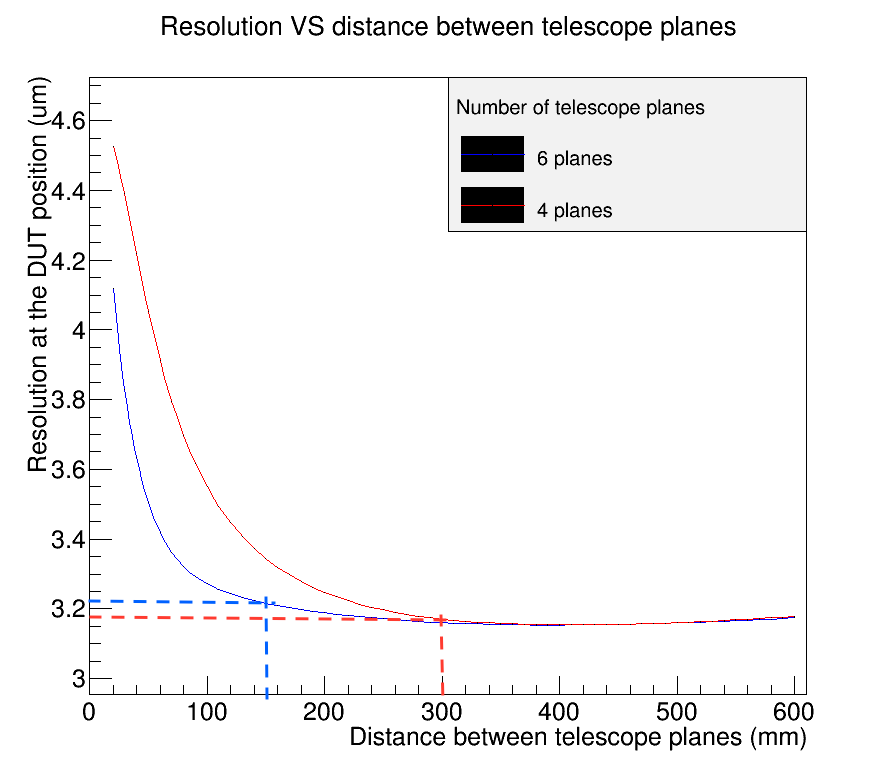
\includegraphics[width = 0.7\textwidth]{Pictures/X0/resolution_4Vs6planes_4-7GeV.png}
      \caption{Estimation of the resolution measured at the DUT position as a function of the distance between two telescope planes of the same arm.
      The blue lines is the results for six planes, whereas the red line is for four planes. 
      The dashed lines are the maximal distance between two planes due to the rail limitation of the telescope frame.}
      \label{fig:estimationRes4.7GeV}
    \end{figure}

    As the number of telescope planes does not impact the pointing resolution, it has been decided to use only four telescope planes and two \gls{PLUME} sensors (one on each side) to simplify the acquisition system.
    %The sensors of the telescope and \gls{PLUME} are both \gls{MIMOSA}-26 thinned down to $50~\rm{\mu m}$.
    %Instead of building a DAQ compatible with EUDAQ, two EUDET telescope planes are removed from the set-up and replaced by two \gls{PLUME} sensors (one on each side).
    However, the synchronisation and the stability of the acquisition have to be tested before the test beam campaign. 

    \subsection{Acquisition system and experimental set-up}
      
      \subsubsection{EUDAQ}

      EUDAQ is a modular cross-platform data taking framework developed for the EUDET-type beam telescopes\cite{Jansen}.
      It is designed to be flexible and to have an easy integration of other devices.
      The software is based on \textit{producers}, that are linked between the different subdetector systems, such as the beam telescope, the \gls{DUT} user DAQ and the \gls{TLU}\cite{Cussans2009}.
      The events of each subdetector are then correlated to form one single global event for data belonging to one trigger.
      This step is done by the \textit{Data Collector}.
      The robustness of the acquisition set-up planed is tested by performing multiple runs for multiple configuration in the laboratory.
      The data are acquired with only the \gls{PLUME} to ensure that EUDAQ can cope it, and then single \gls{MIMOSA}-26 sensors are added and runs of several hours are performed to look for a loss of synchronisation.

      \subsubsection{Experimental set-up}

      Finally, the integration of \gls{PLUME} for the different measurements to perform is investigated.
      For the deformation studies, the \gls{DUT} is mounted on a rotation stage. 
      With respect to the local coordinate system (or sensor coordinate system), the rotation is along the $u$-direction. 
      The first option considerer to performer the rotation is to orient the ladder in the same direction as the telescope's sensors. 
      Hence, the ladder is in the horizontal position and the rotation needs a complicated frame to ensure the stability of the system.
      The weight of the box and ladder is applied only on the rotation stage. 
      Due to the complexity and the time needed to build this frame, a second option has been considered.
      The ladder is placed vertically on a rotation stage. 
      There is a $90^{\circ}$ rotation between the telescope sensors and the \gls{PLUME} ones.
      The frame consists of an insulated aluminum plate on which the \gls{DUT} sits.
      To avoid to damage the \gls{DUT} during the test beam, the flex-cable is maintained on the frame by two clamps.
      In this way, less constraint are applied on the connector. 
      A plate with screws hold the ladder strongly to the frame.
      The frame is then mounted onto a rotation stage, which is mounted on a translation stage.
      The figure~\ref{fig:mechanics} shows a schematic model of the frame designed and built at DESY.
      
      \begin{figure}[!h]
        \centering
        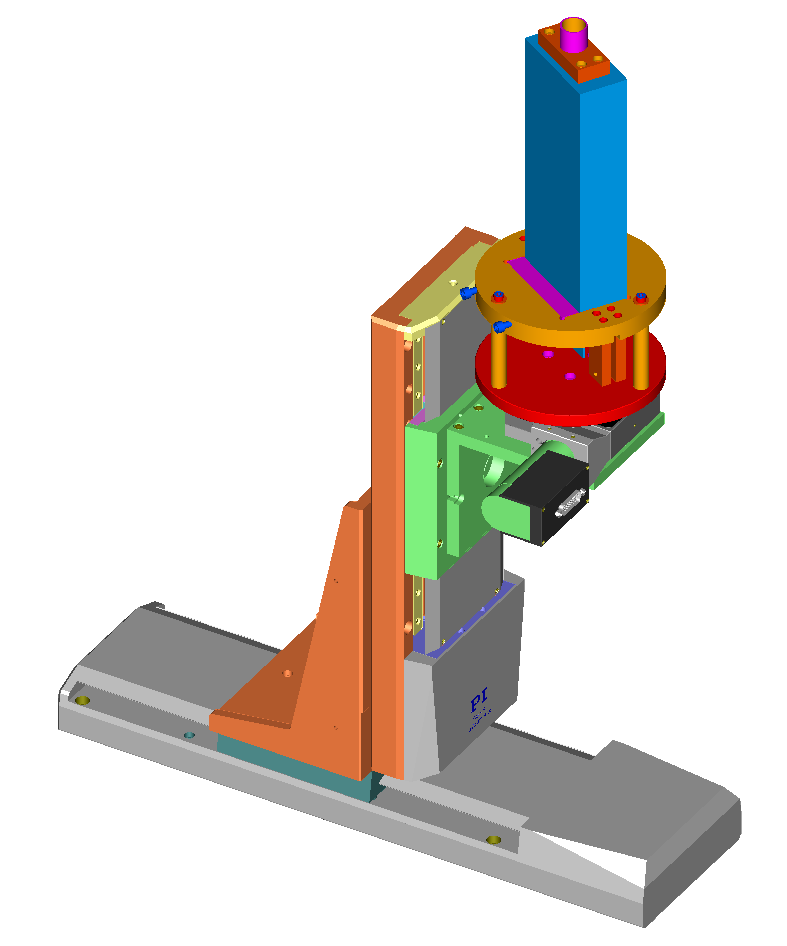
\includegraphics[width = 0.5\textwidth]{Pictures/X0/Frame/Testbeam1.PNG}
        \caption{TCAD model of the mechanical structure designed for the test beam in April. The ladder is hold on a circular frame fixed to a PI rotation stage, mounted onto a XY-table.}
        \label{fig:mechanics}
      \end{figure}

      To control the heating of the ladder during the test beam, a cooling system consisting of a simple fan is used.
      On one endcap, a pipe is fixed and connected to the fan.
      Some studies in Strasbourg were done to determine the air flow speed as a function of the voltage applied.
      Hence, an air flow speed of $3~\rm{m.s^{^1}}$ is achieved with $5~\rm{V}$ and an air flow speed of $6~\rm{m.s^{-1}}$ for $10~\rm{V}$.
      This values result in an operating temperature of all sensors between approximately $40^{\degree}\rm{C}$ and $52^{\degree}\rm{C}$.

      During the test beam campaign, the \textit{clock} and \textit{marker} are read from one sensor of \gls{PLUME}.
      The \textit{clock} is extended with a $80~\rm{cm}$ long cable to ensure that one frame starts on the rising edge.
      The second input of the acquisition is a \gls{PLUME} sensor (opposite side of the first sensor), followed by the four telescope planes. 
      Moreover, \gls{PMT}s are placed in coincidence on each side of the telescope.
      They are used to trigger the acquisition only when the beam passes through the entire set-up.
      Hence, the fake events are reduced and the data stream is smaller.

      %To ensure the synchronisation of the ladder and the telescope planes, the acquisition is synchronised on the \textit{clock} provided by one of the \gls{PLUME} sensor.
      %In the lab, two MIMOSA-26 sensors and the ladder to test are plugged together to the NI-crate. 
      %Runs of several hours are launched to verify the synchronisation.
      %As the \gls{DUT} and telescope planes are connected to the same \textit{JTAG} card and \textit{clock} distribution board, the start signal arrives at the same time on each sensor.
      %If a delay appears, there is a loss in the synchronisation and the acquisition does not work anymore.
      %The frame-counter should be the same on each sensor.

    \begin{figure}[!h]
      \centering
      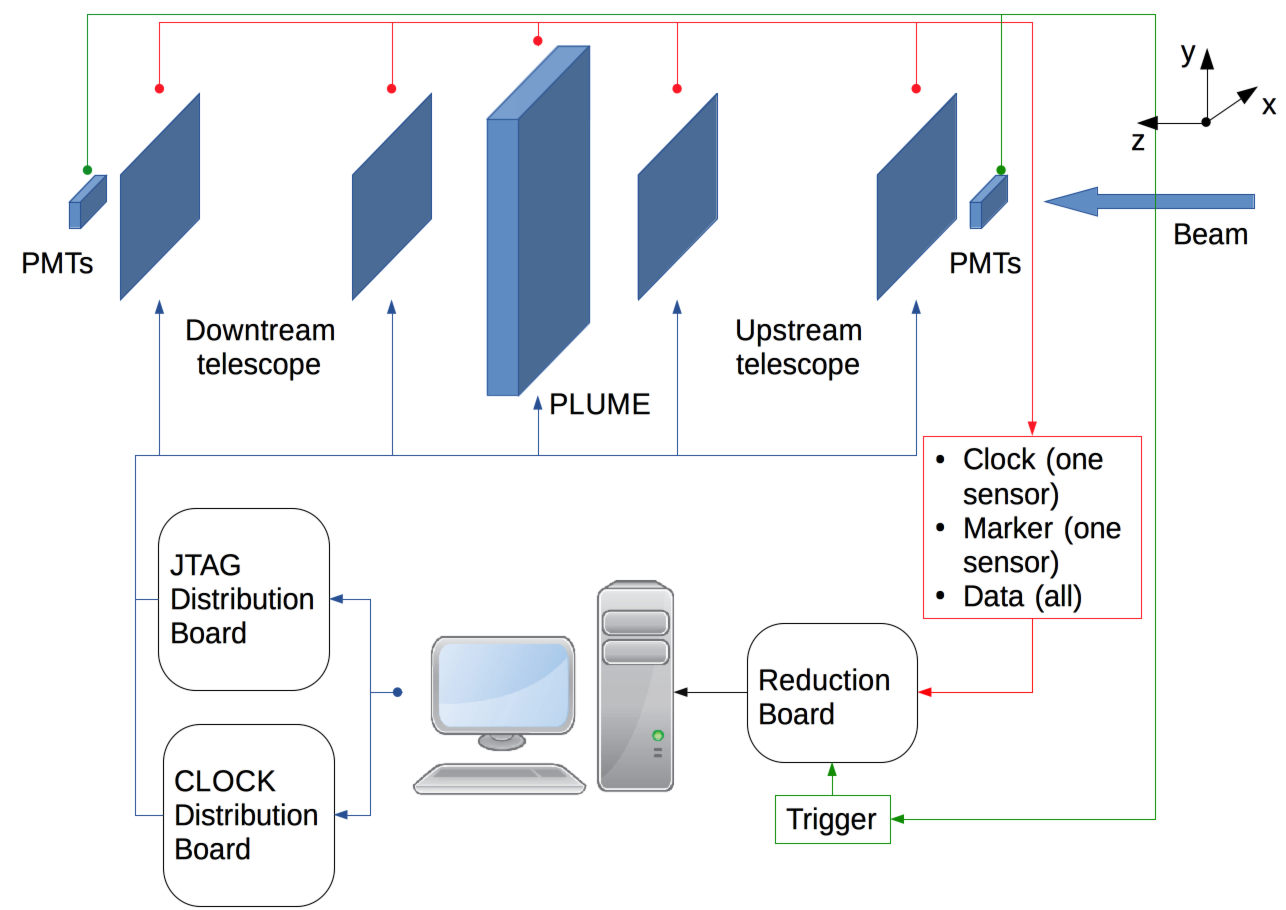
\includegraphics[width = \textwidth]{Pictures/X0/testBeamAcquisition.png}
      \caption{Schematic of the test beam set-up. The PMTs are used for triggering. The clock and marker are read from only one sensor, here it comes from one PLUME sensor.}
      \label{fig:testBeamAcq}
    \end{figure}

    \begin{figure}
      \centering
      \includegraphics[width = 0.8\textwidth]{Pictures/X0/testBeam.png}
      \caption{Picture taken during the test beam. The beam is going out of the magnet before to reach the four telescope planes, the DUT and the PMTs. The set-up is mounted on a floating frame insuring the grounded.}
      \label{fig:testBeam}
    \end{figure}

   
  \section{Measuring the radiation length}

    \subsection{Introduction}
    
    When charged particles are traveling through matter, they lose energy via inelastic collision with atomic electrons and this leads to the ionisation or excitation of the matter.
    Furthermore, along their path, they are deflected by many small angles from their initial trajectory due to Coulomb scattering from nuclei. 
    This stochastic effect, called multiple Coulomb scattering, leaves on the average the particle undisturbed through its path. 
    For small angles of deviation, the multiple scattering is following a Gaussian behavior, whereas for larger angles, it behaves like the Rutherford scattering.
    The Highland formula, which is an empirical formula, describes the distribution of the multiple scattering, or the "kink angle" as a function of the momentum $p$ of the incoming charge particles, its velocity $\beta c$, its charge number $z$ and its true path length in radiation length unit $\frac{x}{X_{0}}$:

    \begin{equation}
      \theta_{0} = \frac{13.6~\rm{MeV}}{\beta c p} z \sqrt{\frac{x}{X_{0}}}\left(1 + 0.038 \ln{\frac{x}{X_{0}}}\right).
      \label{eq:Highland}
    \end{equation}

    For the electrons, a modified version of the equation~\ref{eq:Highland} describes its scattering better than the Highland formula\cite{GEANT4}.

    \begin{equation}
      \theta_{0} = \frac{13.6~\rm{MeV}}{p}\left(\frac{x}{X_{0}}\right)^{0.555},~\text{with $\beta c = 1$.}
    \end{equation}

    The spread angle $\theta_{0}$ depends on the momentum of the incoming particle, as well as the relative radiation length $\frac{x}{X_{0}}$.
    Thus, for a given relative radiation length, the kink angle is becoming smaller for higher momentum, and for a given momentum, this kink angle is not the same for different relative radiation lengths.

    \subsection{Motivation}

    The design of a detector is driven by its intrinsic characteristics, such as the pointing resolution or the integration time, but also by some requirements on the material budget.
    For example, the \gls{ILC} sets new goals for the design of the vertex detector, but also for other parts of the detector, as mentioned in chapters~\ref{chap:ILC} and~\ref{chap:vxd}.
    For such detector, the tracking system should detect precisely the particles path and minimise their energy degradation, while the calorimeters have to measure accurately the energy deposited by the particles.
    During the physics analysis, the reconstruction of the events depends strongly on the knowledge of the energy loss by the particles inside the different components of the detector before they reach the calorimeters. 
    To improve the results, a correction on the energy as to be applied.
    Thus, the study of the radiation length $\rm{X_{0}}$ in $\rm{g.cm}^{2}$, which is the amount of matter traversed by the electron is an important part of the detector development.
    For electrons and positrons, the radiation length corresponds to the mean distance over which these particles loss $1/e$ of its energy by bremsstrahlung.

    As detector are made of different layers, the radiation length for composite materials is given as:

    \begin{equation}
      \frac{1}{X_{0}} = \sum_{j} \frac{\omega_{j}}{X_{j}},
    \end{equation}

   where $\omega_{j}$ and $X_{j}$ are the fraction by weight and radiation length for the $j^{\rm{th}}$ element.


    \subsection{The DESY II test beam facility}

    The \gls{DESY} test beam facility is composed of three areas.
    Firstly, the electron beam is produced in the LINAC-II and accelerated up to 450 MeV before to be injected in the DESY-II synchrotron ring.
    The DESY-II is used as a storage ring for the PETRA-III accelerator. 
    The beam is accelerated and stored until enough particles are available to be sent on to PETRA, where they are used for photon science.
    
    \begin{figure}[!h]
      \centering
      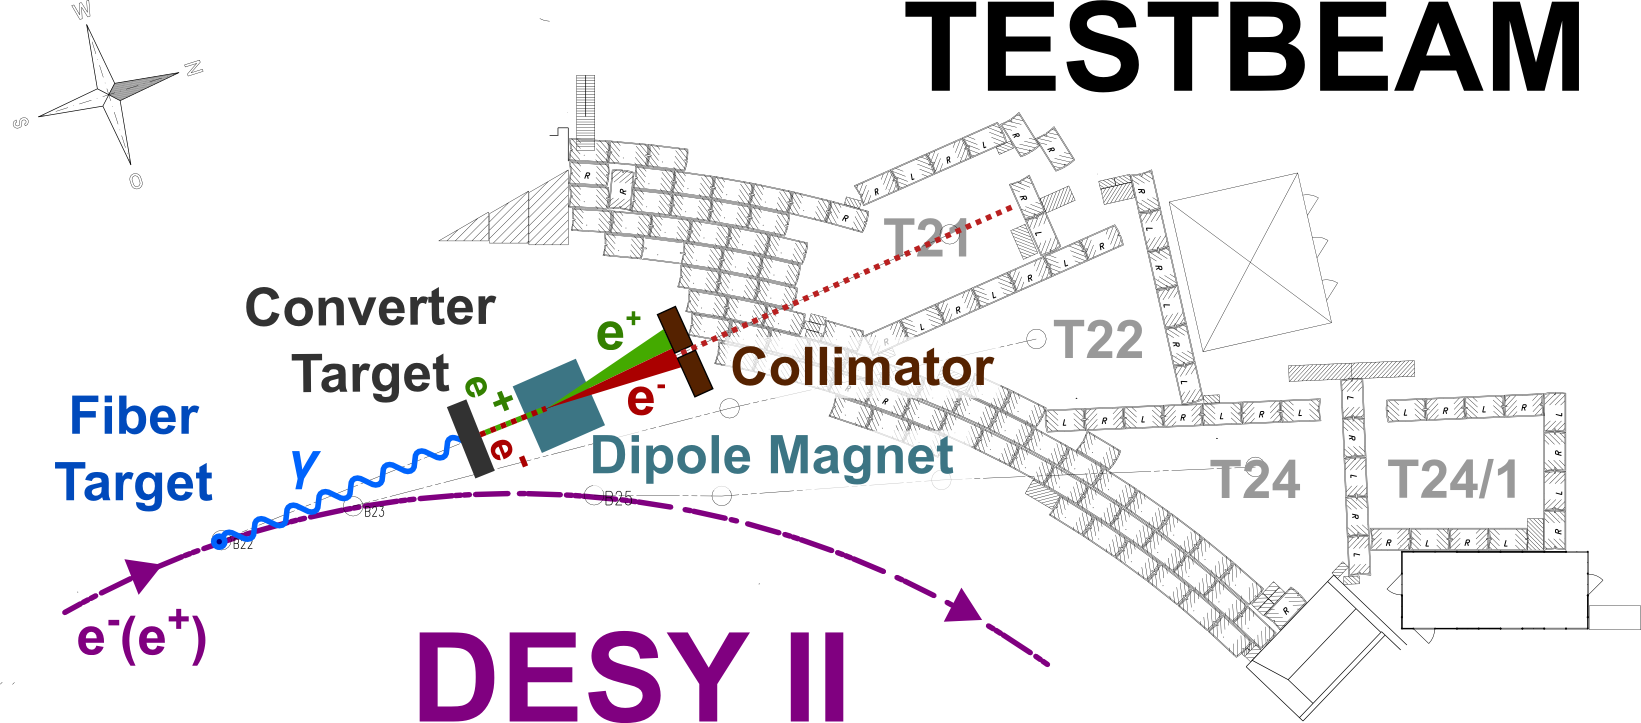
\includegraphics[width = 0.8\textwidth]{Pictures/X0/desy_tb-sketch.png}
      \caption{Schematic layout of the DESY-II test beam facility\cite{DESYII}.}
      \label{fig:desyTb-sketch}
    \end{figure}

    To generate the beam delivered in the Hall 26, a graphite fiber target is placed inside the beam pipe.
    While the electrons are hitting the target, they lose energy and emit bremsstrahlung photons.
    The photons travel through the air and hit another target, on which the photons are converted to pairs of electrons and positrons.
    Different targets with different thicknesses are available and this will impact the particles rate.
    One is made of copper, whereas the other one is made of aluminum.
    Then, a dipole magnet bends the particles and spread them according to their energy.
    Afterward, a tungsten collimator cuts away the unwanted particles, those having a too high or too low momentum, before the test beam area.
    A second collimator is located in the test beam area and it determines the size of the beam spot.
    The figure~\ref{fig:desyTb-sketch} summarises the different step to generate a beam of electrons or positrons in test beam 21, while the energies and the rates available are displayed in figure~\ref{fig:rateTB21}

    \begin{figure}[!h]
      \centering
      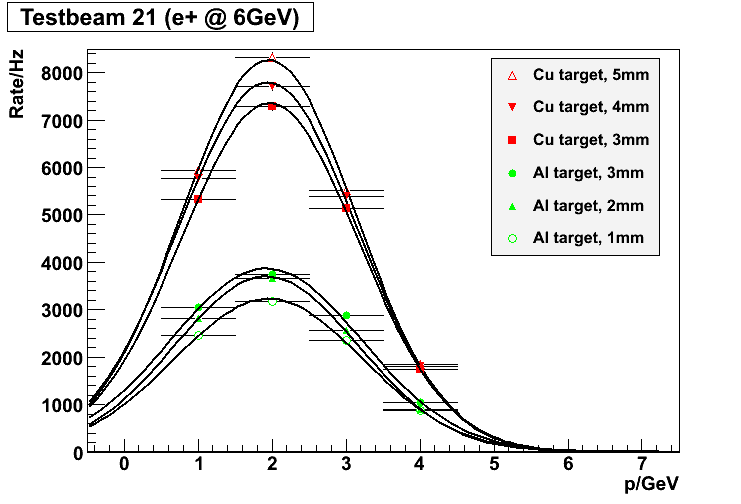
\includegraphics[width = 0.8\textwidth]{Pictures/X0/rate_vs_p_t21.png}
      \caption{Rate for different momentum and with different converter targets\cite{DESYII}.}
      \label{fig:rateTB21}
    \end{figure}


  \section{Analysis}
  \label{sec:X0}

   \subsection{Software analysis chain}

    The analysis of the test beam data is performed with EUTelescope\cite{Eutel}\cite{Jansen}.
    It is based on the MARLIN framework, which is a part of the ILCSOFT (see~\ref{subsec:ILCSOFT} for more details about the ILCSOFT package).
    The software is used to convert the data into the LCIO format and to perform clustering search, alignment and final analysis.
    Each step of the analysis is driven by a dedicated processor.

    A first processor is used to convert the raw data files acquired during the test beam into the LCIO format.
    The new file created contains the pixel number which fired in a given event, along with the sensor number.
    During the conversion, a hot pixel search is done to removed the noisy pixels from the list of hits.
    A pixel is considered as noisy if its firing frequency is above $0.001~\%$
    %From the raw data files, a first processor is used to convert the data into the LCIO format.
    %This converter file contains the pixel number which fired in a given event, along with the sensor number.
    %Before searching for clusters, the noisy pixels are removed from the list.
    %A pixel is considered as noisy if its firing frequency is above a certain value. 
    The noisy pixels correspond to defect raw or column or single pixels always sending information (see section~\ref{sec:noiseMeasurements}).
    Then, a cluster algorithm forms sets of cluster from the adjacent fired pixels in a row and/or column.
    Afterward, the hit candidates are defined with a centre-of-gravity method and the position of the hit is determined in the telescope frame and in the sensor frame.

    Although the alignment procedure looks like the one presented in chapter~\ref{chap:deformation}, the procedure used with EUTElescope is slightly different.
    The alignment is performed with \gls{GBL} and MILLEPEDE-II.
    In the case of a complete telescope (six planes), the tracks are built from the reconstruction of triplets in the upstream and downstream telescope planes.
    Firstly, a hit candidate from the outer plane is extrapolated by a straight line to the inner plane of one arm.
    Then, a triplet is formed if there is a matching between the middle plane of the arm and the doublet built.
    This is done on the two arms and a criterion ensures that two triplets are coming from the same track if the distance between the two extrapolated triplets at the middle $z$-position of the telescope is below a cut value.
    \gls{GBL} form a track from the six hits belonging to the matching triplets.
    The track candidates are then passed to MILLEPEDE-II, which determines the shift and the rotation to apply for aligning the sensors.
    This method is applied a couple of times, until the precision of the alignment reaches a submicron order.

    Nevertheless, due to the set-up used during the test beam and a limitation in EUTElescope on the number of telescope planes and the ID used, the alignment did not work.
    Indeed, the number of telescope planes is hard-coded to be six and the sensor IDs in the range $[0; 5]$ are reserved for the telescope. 
    Here, the IDS $0$ and $1$ are used for \gls{PLUME} and the others for the telescope.
    Thus, a modification has to be applied to remap the sensor IDs. 
    Although this solution can work and \gls{GBL} uses only the $z$ ordering information is used to create the tracks, EUTelescope is waiting for six hits.

   % For the upstream and the downstream plane, a hit position from the outer plane is projected on the inner plane with a straight line. 

   % Almost the same procedure as presented in chapter~\ref{chap:deformation} is performed, except that the alignment is done with \gls{GBL}.

   % Nevertheless, for my set-up, the alignment step did not work.
   % Inside EUTelescope, the number of telescope planes is hard-coded to be six and the sensor IDs in the range $[0; 5]$ are only for the telescope.
   % These IDs have to be ordered according to the $z$-direction too.
   % In my case, the IDs $0$ and $1$ are used for \gls{PLUME} and the rest for the telescope. 
   % Although \gls{GBL} uses only the $z$-ordering information to perform the alignment, the alignment procedure never worked.

    Thankfully, a prototype software developed by Claus Kleinwort has permitted to perform the alignment and finish the analysis. 
    It is based on \gls{GBL} and MILLEPEDE-II and reads the hit information created by the hitmaker processor of EUTelescope. 
    The modularity of the software allows to select the desire number of telescope planes.
    In the case of only four telescope planes, the triplets method is not used and tracks are formed only with doublets.
    Then, the track's information are feed to MILLEPEDE-II, which calculates the residuals of the tracks on each sensor and attempts to shift the position and rotate the sensors to minimise the east square fit function of these tracks.
    MILLEPEDE-II creates an output file with theses informations and a script update the GEAR file with the new position and orientation of each planes.

    %Then, the subtrack is extrapolated to the middle plane of the arm and \gls{GBL} is looking for the closest hit to the subtrack candidate.
    %This tracks are called triplets.
    %Afterward, the software finds if triplets are converging at the \gls{DUT} position and form a single track, unless multiple triplets are connected at the same position.
    %In this case, the track is rejected.

    %The tracks created are then read by Millepede-II, which calculates the residuals of the tracks on each sensor and attempts to shift the position of the sensors and to rotate them in order to minimise the least squares fit function of these tracks.
    %Millepede-II provides these informations into an output file used to create a new GEAR file with the new position and orientation of each plane.
    
    \begin{figure}[!h]
      \centering
      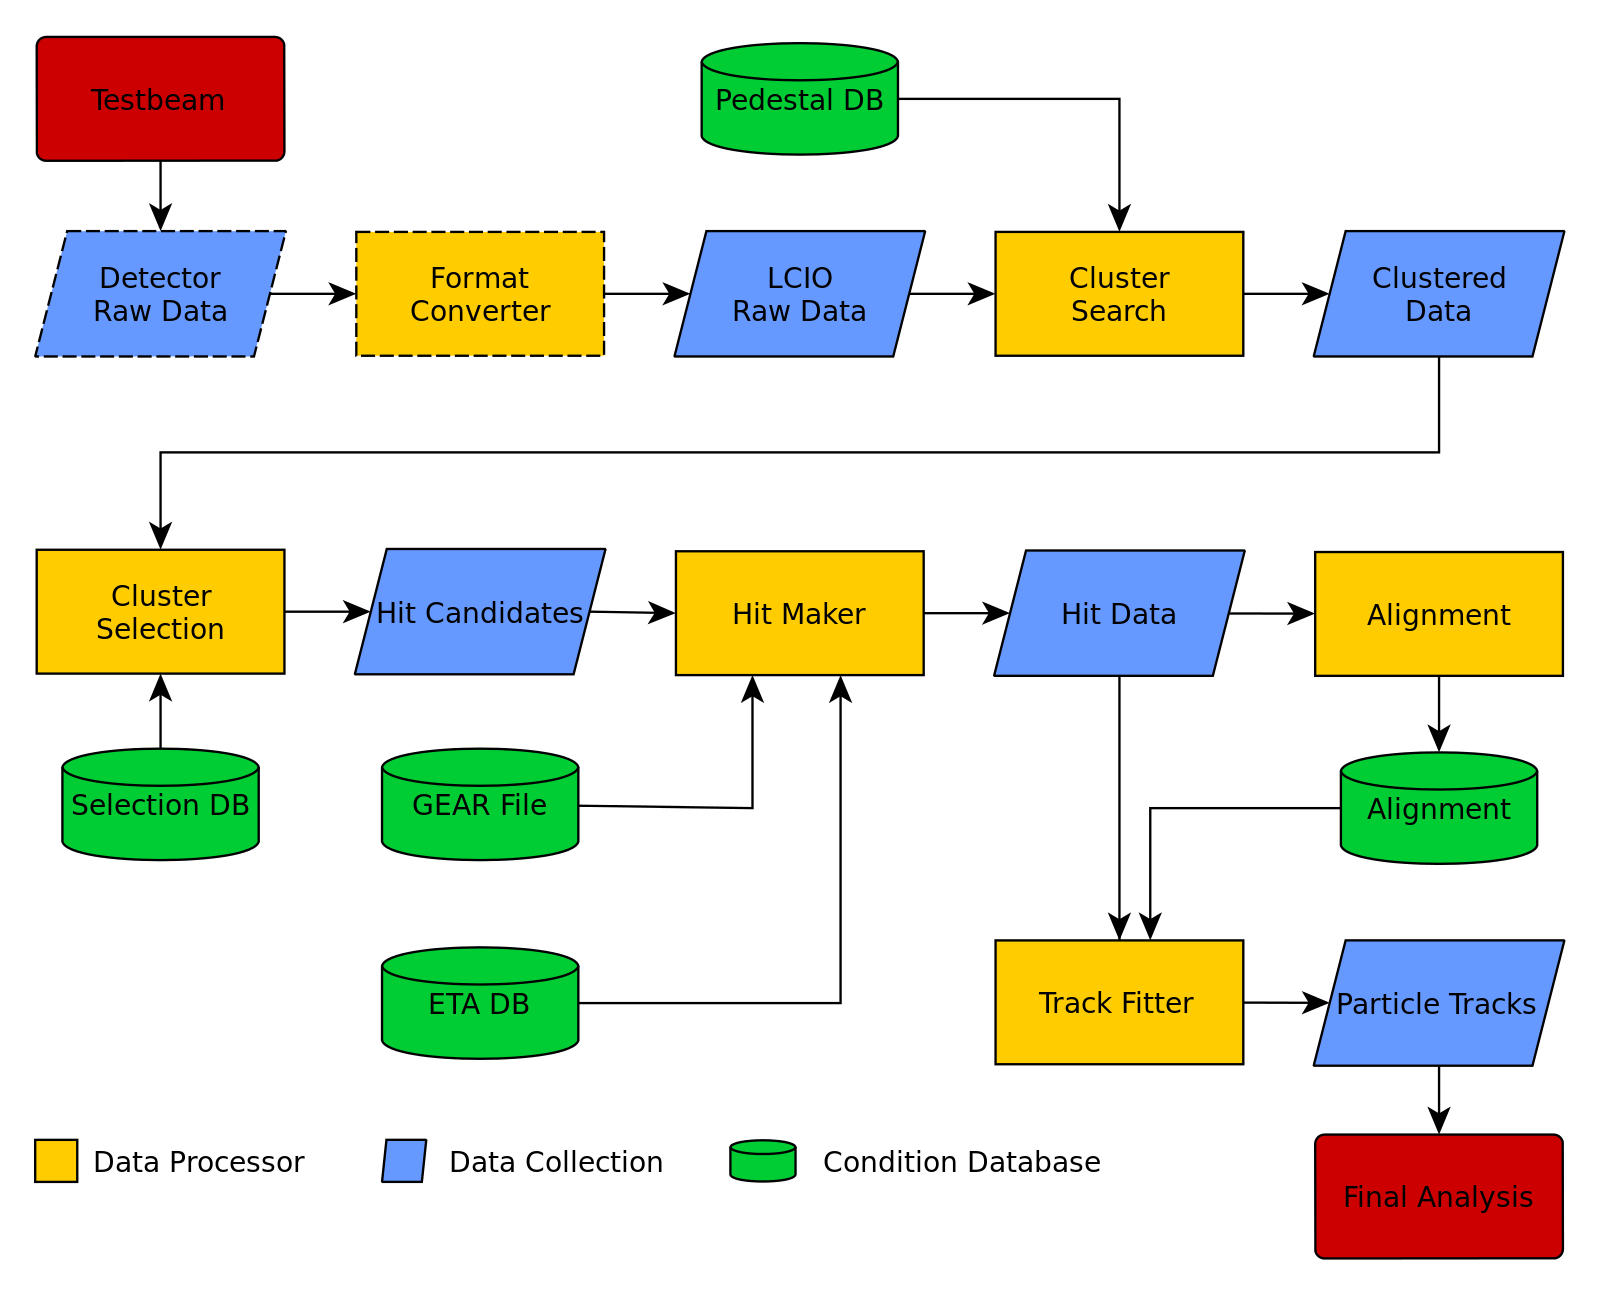
\includegraphics[width = \textwidth]{Pictures/X0/eutel-strategy.png}
      \caption{Flow-chart of the analysis strategy by using EUTelescope.}
      \label{fig:eutel-strategy}
    \end{figure}

   \subsection{Measurement of the radiation length}

   To extract the radiation length a biased alignment is performed.
   The hit information of \gls{PLUME} are used to create tracks by using the triplets method.
   The deviation of the track between its position before \gls{PLUME} and after \gls{PLUME} is measured with \gls{GBL}, that provides information for $xz$ and $yz$-angles.
   The distribution of the kink angle is fitted by a Gaussian, as represented on figure~\ref{fig:kinkAngle} for an energy of $5~\rm{GeV}$.
   The distribution displayed here is the kink angle measured on all the reference planes, no fiducial cut was applied. 

%
%   The extraction of the radiation length is done by measuring the kink angle between the track reconstructed before the \gls{DUT} and the track reconstructed after.
%   \gls{GBL} provides this information for $xz$ and $yz$-angles.
   %For the results presented here, a track is made of six hits: four coming from the telescope planes and two from the \gls{PLUME} sensors.
   %The distribution of the kink angle is fitted by a Gaussian, as represented on figure~\ref{fig:kinkAngle} for an energy of $5~\rm{GeV}$.
   Here, no fiducial cut has been applied and the measured kink angle is done on the overlapping region between the telescope and the \gls{DUT} planes.
   As it can be seen, the fit is not performed on the full range because of tails due to systematic errors.
   The measured kink angle is done for the energy range $[1; 5]~\rm{GeV}$ with a step of $1~\rm{GeV}$.
   The figure~\ref{fig:theta0vsP_all} displays the kink angle measured as a function of the particles momentum.
   The uncertainty on the momentum is $5~\%$ and is the uncertainty determined at the DESY test beam facility, while the uncertainty used for the kink angle is extracted from the fit procedure.
   The plot is then fitted with the Highland formula, on which the radiation length is a free parameter.
   The fit result is not convincing.
   Two points ($1$ and $5~\rm{GeV}$) are excluded and the $\chi^2 /~\rm{N.D.F}$ measured is bigger than $1$.
   Nevertheless, the $5~\rm{GeV}$ measurement gives a radiation length of $\sim 0.65~\%~\rm{X_{0}} $.

   During the alignment procedure, the runs at $1$ and $2~\rm{GeV}$ were complicated to be done.
   At those energies, the electron are more sensitive to the multiple scattering in the air and inside the detectors.
   By excluding the $1~\rm{and}~2~\rm{GeV}$ measurement, the radiation length is $x/X_0 \simeq 0.53~\%~\rm{X_{0}}$ and the $\chi^2$ is closer to one.

   %After the alignment step is done, the extraction of the radiation length from the reconstructed data can start.

   %Firstly, the angle between the track reconstructed by the upstream and the downstream telescope arms is studied.
   %\gls{GBL} is providing this information for $xz$ and $yz$-angles.
   %The distribution is fitted by a Gaussian, as seen on figure~\ref{fig:kinkAngle}.
   %As it can be seen, the fit is not performed on the full range because of tails due to systematic errors.
   %The measured kink angle is done for different energies to extract the radiation length.
   
   \begin{figure}
     \centering
     \missingfigure{Kink angle distribution}
     \caption{Distribution of the kink angle given by GBL for an energy of $5~\rm{GeV}$ without any fiducial cut.}
     \label{fig:kinkAngle}
   \end{figure} 

   %This measurement was performed at $5~\rm{GeV}$ and by using the Highland formula, the material budget determined is $\sim 0.6~\%~\rm{X_{0}} \pm $.

   %A sanity check is done for energies from 1 to $4~\rm{GeV}$.
   %The same procedure is applied and the distribution of the kink angle measured as a function of the momentum of the beam is plotted and fitted by the Highland formula to determine the radiation length of the \gls{DUT} (see~\ref{fig:theta0vsP}).
   %The uncertainty on the momentum is set to $5~\%$ and is the uncertainty measured at the DESY test beam facility, while the uncertainty used for the kink angle is extracted from the fit procedure.
   %Nonetheless, the fit results is bad and the measured radiation length is $x/X_0 \simeq 0.48~\%~\rm{X_{0}}$.
   %The measured radiation length is below the theoretical expectation but other tests have to be performed before to conclude.

   %The radiation length depends only on the material and not the energy.
   %Nevertheless, the figure~\ref{fig:X0vsP} which represents the measured radiation length as a function of the momentum, gives a $\rm{X_{0}}$ depending on the momentum.
   %So, the $0.53~\%~\rm{X_{0}}$ measured are likely to be wrong.

   %The error could emerge from the small analysis software to produce the plots.
   %To check the exactness of the code, the 

   \begin{figure}
     \centering
     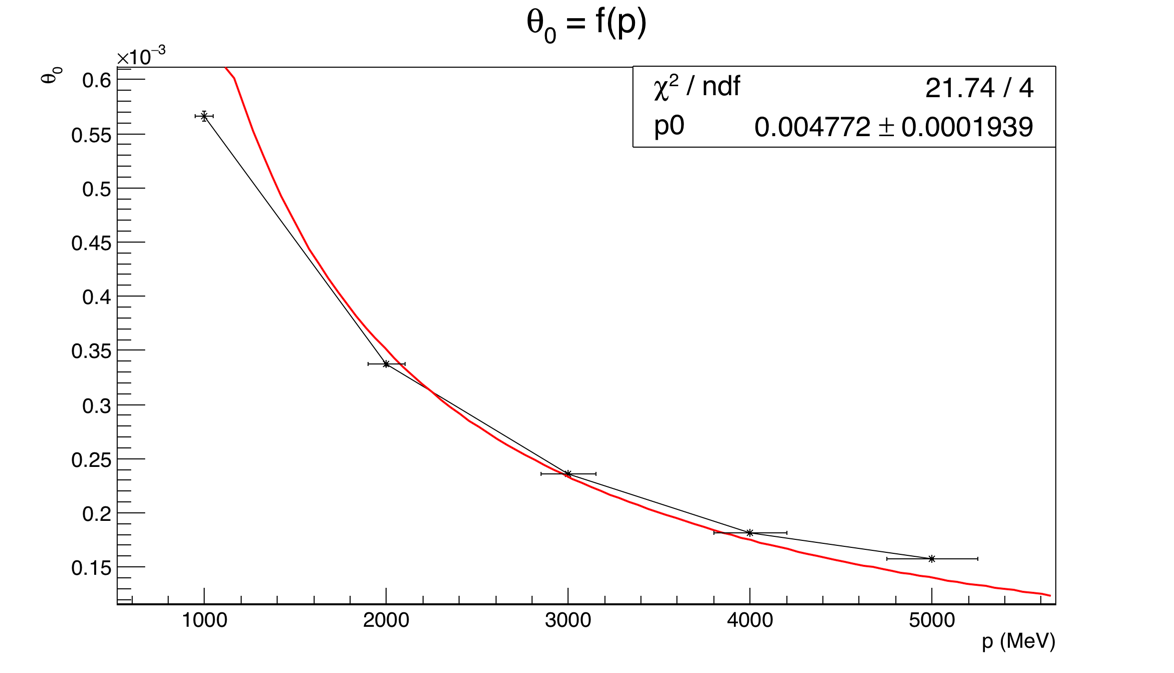
\includegraphics[width = \textwidth]{Pictures/X0/theta0VsP_all.png}
     \caption{Extrapolation of the measured radiation length with a fit between 1 and 5 GeV.}
     \label{fig:theta0vsP_all}
   \end{figure}
   \begin{figure}
     \centering
     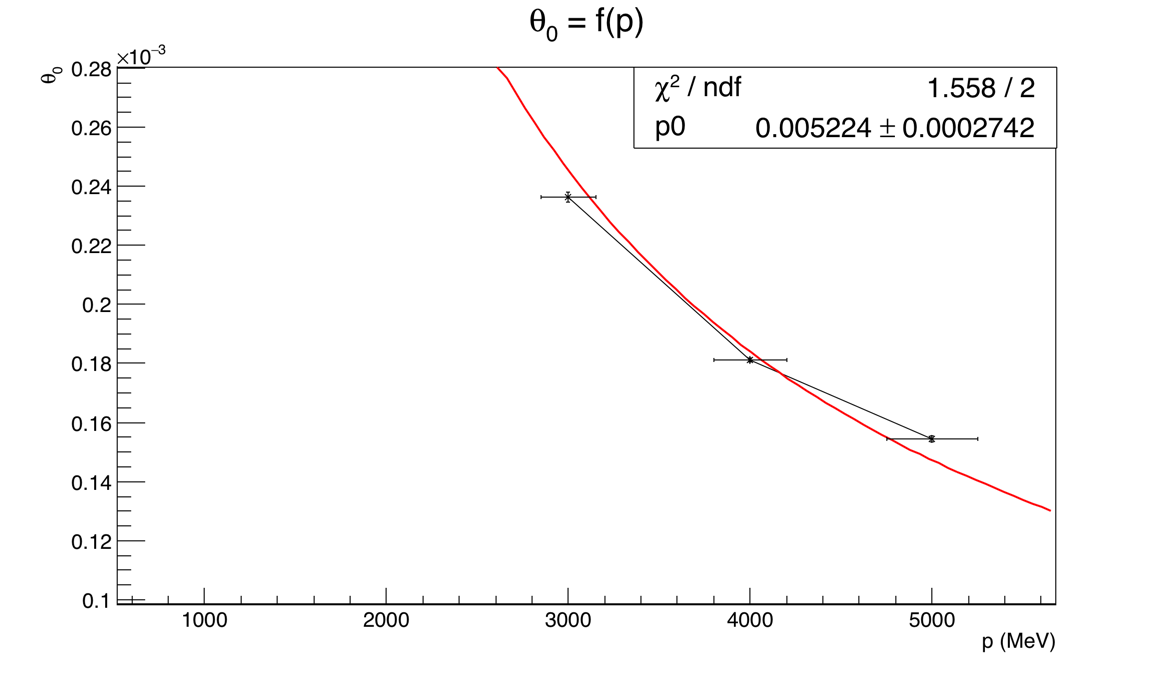
\includegraphics[width = \textwidth]{Pictures/X0/theta0VsP_3-5GeV.png}
     \caption{Extrapolation of the measured radiation length in the range 3 to 5 GeV.}
     \label{fig:theta0vsP_3-5}
   \end{figure}

   \begin{figure}
     \centering
     \missingfigure{x/X0 Vs energy}
     \label{fig:X0vsP}
   \end{figure}


  \section{Conclusions}

  The radiation length measurement of the \gls{PLUME} ladder was performed for the first time and the results are not good enough to conclude if the material budget determined theoretically for the first fully functional ladder is correct.
  To improve the measurement, it could be useful to perform calibration runs with a known material to check that the analysis is working correctly.
  Moreover, a correction can be performed then on the measured material budget with \gls{PLUME}.

  During the test beam and the data analysis, there was several problems.
  Firstly, due to a broken component on the power distribution board, one side of \gls{PLUME} was not working correctly.
  The sensors were sending the \textit{header} and \textit{trailer} but no data information, leading to two days of fully test before to find the origin of the problem.
  Fortunately, after replacing the broken component, the ladder was working normally but it is likely that the thresholds set were not correct anymore.
  Nevertheless, the data could have been corrupted and this should be investigated.

  Besides the analysis was complicated.
  EUTelescope is expecting a certain sensor IDs order and six telescope planes, even if \gls{GBL} is working from three to a huge amount of plane.
